\section{Einleitung}
Der Bereich der IT-Security hat in den letzten Jahren zunehmend an Bedeutung gewonnen, was vor allem auf die steigenden Fallzahlen von Cyberkriminalität zurückzuführen ist. Insbesondere Vorfälle großer Datenverluste bei namhaften Unternehmen rücken das Thema in den medialen Fokus und schaffen ein wachsendes Bewusstsein für die Bedeutung der Cybersicherheit. Dies hat eine steigende Nachfrage nach effektiven Lösungen zur Sicherung digitaler Infrastrukturen und deren Überwachung zur Folge.

Im Kontext der Überwachung von Netzwerken entstehen bereits in kleinen Infrastrukturen riesige Datenmengen, die von Menschen nicht in akzeptabler Zeit ausgewertet werden können. Diese Herausforderung führt dazu, dass wertvolle Informationen nicht aktiv zur Verbesserung der Netzwerksicherheit genutzt werden können. Eine vielversprechende Lösung zur Bewältigung dieses Problems ist der Einsatz von \ac{SOAR}-Systemen. Diese Systeme unterstützen Sicherheitsteams dabei, Sicherheitsereignisse effektiv zu orchestrieren und automatisieren.

\ac{SOAR}-Systeme ermöglichen \cite{PICUS.2023} die kontinuierliche Überwachung von Netzwerken und sind mittlerweile ein integraler Bestandteil von Security Operation Centern. Sie aggregieren Ereignisse aus verschiedenen Quellen und stellen diese in Echtzeit dar, was die Effizienz der Sicherheitsoperationen erheblich steigert und eine Automatisierung ermöglicht. Angesichts der kritischen Rolle, die solche Systeme in der IT-Infrastruktur von Unternehmen spielen, ist eine fehlerfreie Funktionsweise unerlässlich. Zudem müssen \ac{SOAR}-Systeme robust gegenüber Angriffen sein und eine geringe Fehleranfälligkeit aufweisen, um den Anforderungen an moderne Sicherheitsarchitekturen gerecht zu werden.

\begin{comment}
\subsection{Zielsetzung}
Kleiner Reminder für mich in Bezug auf die Dinge, die wir bei der Thesis beachten sollten und \LaTeX{}-Vorlage für die Thesis.

\subsection{Aufbau der Arbeit}
Kapitel \ref{infos} enthält die Inhalte des Thesis-Days und alles, was zum inhaltlichen erstellen der Thesis relevant sein könnte. In Kapitel \ref{latexDetails} \nameref{latexDetails} findet ihr wichtige Anmerkungen zu \LaTeX{}, wobei die wirklich wichtigen Dinge im Quelltext dieses Dokumentes stehen (siehe auch die Verzeichnisstruktur in Abbildung \ref{fig:verzeichnisStruktur}).


\begin{figure}[H]
\caption{Verzeichnisstruktur der \LaTeX{}-Datein}\label{fig:verzeichnisStruktur}
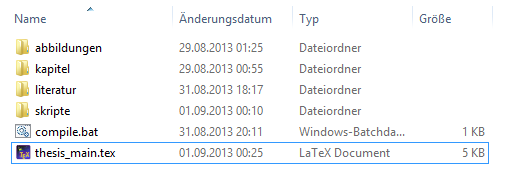
\includegraphics[width=0.9\textwidth]{verzeichnisStruktur}
\\
Quelle: Eigene Darstellung
\end{figure}
\end{comment}